\section{Auswertung}

Bei den folgenden Rechnungen wurden die Messwerte aus den vom XY-Schreiber erstellten
Graphen abgelesen und mittels Python ausgewertet. Bei den Werten wurden Mittelwert
und Standardabweichung des Mittelwerts nach folgenden Formeln ermittelt:

\begin{align}
  \bar{x}      &= \frac{1}{N} \cdot \sum_{i=0}^{N} x\ua{i}
  \label{eqn:Mittelwert} \\
  s\ua{\bar{x}} &= \sqrt{ \frac{1}{N(N-1)} \cdot \sum_{i=0}^{N} (x\ua{i} - \bar{x})^2  }.
  \label{eqn:Standardabweichung}
\end{align}

Die linearen Regressionen bei der Auswertung der verschiedenen Messungen wurden
alle an die selbe Formel gefittet \eqref{eqn:linRegress}, wobei die Parameter
unterschiedlichen physikalischen Größen zugeordnet werden, welche in den einzelnen
Messabschnitten noch einmal erwähnt werden.

\begin{equation}
  f(x) = A \cdot x + B
  \label{eqn:linRegress}
\end{equation}

Bei jeder Messung wurden die Temperaturen möglichst konstant gehalten. Mit den
gemessenen Temperaturen lassen sich gemäß Formel \eqref{eqn:weglänge} und Formel
\eqref{eqn:Sättigungsdruck} die mittlere freie
Weglänge $\bar{w}$ sowie das Verhältnis $\frac{a}{\bar{w}}$ mit dem Abstand zwischen
Kathode und Beschleunigungselektrode $a$ ($a$ = $\SI{1}{cm}$) berechnen.

\begin{equation}
  p\ua{saet}(T) = 5.5 \cdot 10^{7} \exp{-6876/T}
  \label{eqn:Sättigungsdruck}
\end{equation}

Die ermittelten Werte sind in der folgenden Tabelle zu sehen.

\begin{table}
  \centering
  \caption{Aus den Messwerten ermitteltes Ergebniss für $\frac{a}{\bar{w}}$.}
  \label{tab:Weglaengen}
  \begin{tabular}{c c c c}
    \toprule
    $T$ in $\su{K}$ & $p\ua{saet}$ in $\su{mbar}$ & $\bar{w}$ in $\su{cm}$
    & $\frac{a}{bar{w}}$ \\
    \midrule
    300.15 & 0.0062  & 0.4689 & 2.13    \\
    417.15 & 3.8174  & 0.0008 & 1316.34 \\
    459.15 & 17.2420 & 0.0002 & 5945.50 \\
    380.15 & 0.7674  & 0.0038 & 264.62  \\
  \end{tabular}
\end{table}


Zudem wurde bei allen Messungen mithilfe des XY-Schreibers ein X-Achse eingezeichnet,
um die jeweiligen Spannungswerte ablesen zu können. Da die Skaleneinteilung bei
jeder Messung bekannt ist, kann mithilfe einer linaren Regression nach Formel
\eqref{eqn:linRegress} berechnet werden, wieviel Volt ein Millimeter auf dem Graphen entspricht.
Dabei wird die Spannung gegen den Abstand aufgetragen (Tabelle
\ref{tab:Kaestchen}), so dass die Steigung $A$ das
gesuchte Verhältniss wieder gibt.

\begin{table}
  \caption{Der Abstand N in mm und die entsprechende Spannung.}
  \label{tab:Kaestchen}
  \begin{tabular}{c c c | c c c}
    \toprule
    \multicolumn{3}{c}{Messung 3.1)} & \multicolumn{3}{c}{Messung 3.2) und 3.3)} \\
    $U$ in $\su{V}$ & N bei $\SI{300.15}{K}$ & N bei $\SI{417.15}{K}$
    & $U$ in $\su{V}$ & N bei $\SI{459.15}{K}$ & N bei $\SI{380.15}{K}$ \\
    \midrule
    1  &  19 &  20 &  5 &  18 &  19 \\
    2  &  40 &  43 & 10 &  39 &  43 \\
    3  &  61 &  64 & 15 &  57 &  64 \\
    4  &  81 &  84 & 20 &  75 &  85 \\
    5  & 103 & 104 & 25 &  91 & 104 \\
    6  & 123 & 126 & 30 & 110 & 121 \\
    7  & 143 & 146 & 35 & 128 & 142 \\
    8  & 164 & 168 & 40 & 146 & 163 \\
    9  & 185 & 189 & 45 & 165 & 183 \\
    10 & 208 & 211 & 50 & 184 & 201 \\
    11 & 228 & 229 & 55 & 205 & 221 \\
       &     &     & 57 & 215 & 232 \\
    \bottomrule
  \end{tabular}
\end{table}


Die bestimmten Steigungen sind in der folgenden Tabelle zu sehen:

\begin{table}
  \centering
  \caption{Bestimmte Werte für die X-Achsen der verschiedenen Messungen.}
  \label{tab:Steigungen}
  \begin{tabular}{c | c c c c }
    \toprule
    Messungen & 3.1) bei $\SI{300.15}{K}$ & 3.1) bei $\SI{417.15}{K}$ &
    3.2) bei $\SI{459.15}{K}$ & 3.3) bei $\SI{380.15}{K}$ \\
    \midrule
    $A$ in $\frac{1}{\su{V}}$            & 0.0479 & 0.0478 & 0.2696 & 0.2497 \\
    $\sigma\ua{A}$ in $\frac{1}{\su{V}}$ & 0.0002 & 0.0002 & 0.0025 & 0.0019 \\
  \end{tabular}
\end{table}


Da für die Ablesefehler ein Wert von ca. $\SI{0.2}{mm}$ angenommen wird, sind
die dadurch entstehenden Fehler im Bezug auf die Spannung so gering, dass die
abgelesenen Spannungen aus dem Graphen im folgenden als fehlerfrei angenommen werden.


\subsection{Bestimmung der Energieverteilung}

Um die Energieverteilung bei den verschiedenen Temperaturen zu bestimmen, wird
die Steigung der beiden Graphen an verschiedenen Punkten gemessen. Dafür wird immer
die Steigung in einem Intervall von einem mm um den Punkt bestimmt. Die gemessenen
Werte sind in der Tabelle \ref{tab:MessungA27} sowie grafisch in den Abbildungen
\ref{fig:Messung_A_27} und \ref{fig:Messung_A_144} zu sehen.

\begin{table}
  \centering
  \caption{Abgelesene Werte bei Messung 3.1.}
  \label{tab:MessungA27}
  \begin{tabular}{c c |c c}
    \toprule
    \multicolumn{2}{c}{27 °C} & \multicolumn{2}{c}{144 °C} \\
    x in $\su{V}$ & $ \frac{\increment x}{\increment y}$ &
    x in $\su{V}$ & $ \frac{\increment x}{\increment y}$ \\
    \midrule
    0.048  & 62.60 & 0.191 & 125.59 \\
    0.479  & 41.73 & 0.382 & 104.66 \\
    0.958  & 52.17 & 0.573 & 125.59 \\
    1.438  & 41.73 & 0.860 &  83.72 \\
    1.917  & 41.73 & 1.051 & 104.66 \\
    2.396  & 31.30 & 1.338 &  83.72 \\
    2.875  & 41.73 & 1.529 & 104.66 \\
    3.355  & 41.73 & 1.720 &  62.79 \\
    3.834  & 31.30 & 1.911 &  83.72 \\
    4.313  & 31.30 & 2.102 &  62.79 \\
    4.792  & 31.30 & 2.245 &  62.79 \\
    5.272  & 31.30 & 2.437 &  62.79 \\
    5.751  & 20.87 & 2.580 &  41.86 \\
    6.230  & 20.87 & 2.723 &  41.86 \\
    6.709  & 20.87 & 2.867 &  31.40 \\
    6.997  & 31.30 & 3.058 &  52.33 \\
    7.285  & 20.87 & 3.201 &  41.86 \\
    7.524  & 20.87 & 3.297 &  20.93 \\
    7.764  & 20.87 & 3.392 &  20.93 \\
    7.860  & 20.87 & 3.488 &  20.93 \\
    7.955  & 31.30 & 3.583 &  20.93 \\
    8.051  & 41.73 & 3.679 &  20.93 \\
    8.147  & 41.73 & 3.774 &  0  \\
    8.243  & 41.73 & 3.870 &  0  \\
    8.339  & 31.30 & 3.965 &  0  \\
    8.435  & 20.87 & 4.061 &  0  \\
    8.531  & 20.87 & 4.156 &  0  \\
    8.866  & 0     & 4.539 &  0  \\
    9.345  & 0     & 5.064 &  0  \\
    9.872  & 0     & & \\
  \end{tabular}
\end{table}


\begin{figure}
  \centering
  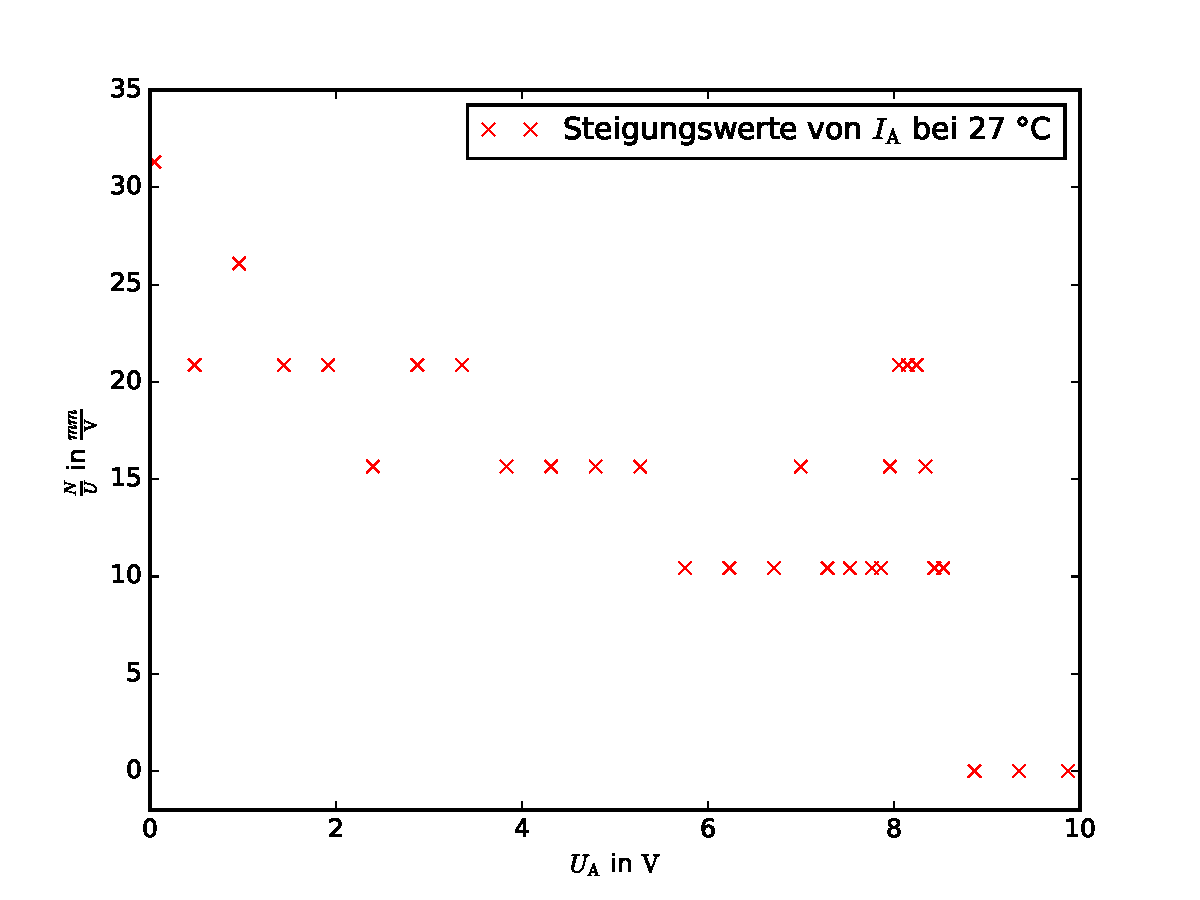
\includegraphics[width = 0.75\textwidth]{Pics/Messung_A_27.pdf}
  \caption{Abgelesene Steigungen bei Messung 3.1 bei 27 °C.}
  \label{fig:Messung_A_27}
\end{figure}

\begin{figure}
  \centering
  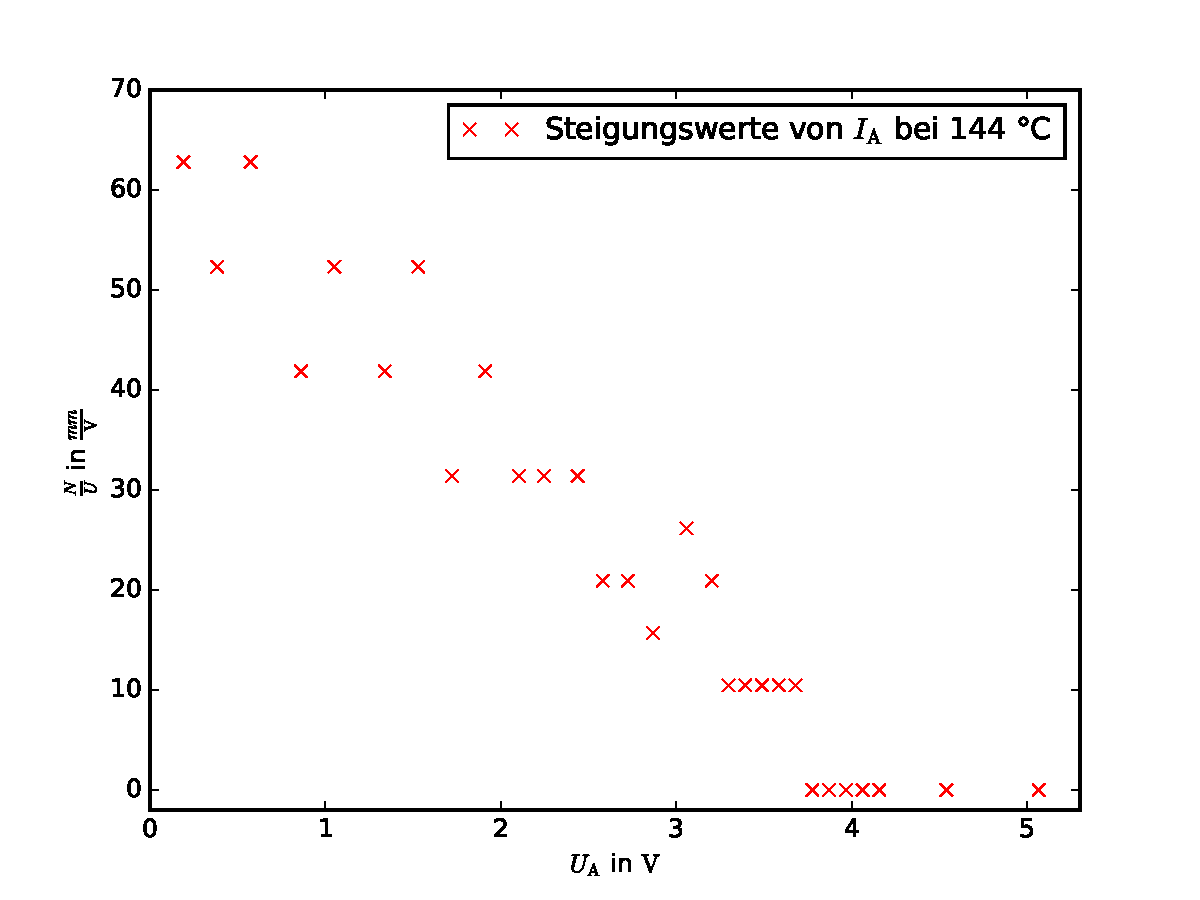
\includegraphics[width = 0.75\textwidth]{Pics/Messung_A_144.pdf}
  \caption{Abgelesene Steigungen bei Messung 3.1 bei 144 °C.}
  \label{fig:Messung_A_144}
\end{figure}

In Abbildung \ref{fig:Messung_A_27} sieht man, dass sich bei $U\ua{B,eff}$ =
$\SI{8.147}{V}$ ein
Piek befindet. Da es sich um die Fermi-Dirac-Verteilung handelt, liegt dieser
Piek theoretisch bei der Beschleunigungsspannung $U\ua{B}$ = $\SI{11}{V}$. An
diesem Punkt ist die Energie der Elektronen gerade so groß, um das Kontaktpotenzial
zu überwinden und die Quecksilberatome anzuregen. Die Elektronen wechselwirken
somit mit den Quecksilberatomen und gelangen nicht mehr bis zur
Auffängerelektrode. Resultierend daraus befindet sich bei $U\ua{B,eff}$ der
stärkste Abfall.
Aus der Differenz dieser beiden Werte kann nun das Kontaktpotential bestimmt
werden:

\begin{equation}
  \su{K}\ua{A} = U\ua{B}- U\ua{B,eff} = \SI{11}{V} - \SI{8.147}{V} = \SI{2.853}{V}.
\end{equation}

Bei dem zweiten Graphen ist so ein Energiemaximum nicht mehr erkenntlich (Abb.
\ref{fig:Messung_A_144}). Dies liegt
an dem Verhältniss $\frac{a}{\bar{w}}$, welches hier deutlich höher ist (siehe
Tabelle \ref{tab:Weglaengen}). Somit treten deutlich mehr elastische Stöße auf,
welche die Richtung der Elektronen beeinflussen. Dies führt zu einer deutlich
geringeren Zahl an Elektronen, die an der Auffängerelektrode registriert werden,
so dass die Energie-Verteilung in Feldrichtung verwischt wird und keinen
Zusammenhang zur Fermi-Dirac-Verteilung mehr zeigt.

Auffällig ist zudem, dass bei der zweiten Messreihe kaum Elektronen mit einer
Energie über $\SI{5}{eV}$ die Auffängerelektrode erreichen. Dies liegt daran,
dass die in 3.2 bestimmte Anregungsenergie von Quecksilber $\SI{5.160 \pm 0.035}{V}$
(\ref{eqn:Anregung}) beträgt. Somit wechselwirken Elektronen mit einer größeren
Energie mit den Quecksilber-Atomen und gelangen aufgrund des Gegenfeldes nicht
mehr an die Auffängerelektrode.


\subsection{Beobachtung der Franck-Hertz-Kurve}

Mithilfe der Franck-Hertz-Kurve soll im Folgenden nun die 1. Anregungsenergie für
Quecksilber bestimmt werden. Dafür werden auf dem Graphen die Abstände zwischen
den Maxima gemessen. Mit Formel \ref{eqn:Mittelwert} wird dann der Mittelwert
bestimmt. Die gemessenen Werte sind in der folgenden Tabelle eingetragen.

\begin{table}
  \centering
  \caption{Gemessene Abstände zwischen den Maxima.}
  \label{tab:AbstaendeMaxima}
  \begin{tabular}{c c}
    \toprule
    $\increment x$ in $\si{mm}$ & $\increment U$ in $\si{V}$ \\
    19 & 5.121 \\
    19 & 5.121 \\
    18 & 4.852 \\
    19 & 5.121 \\
    21 & 5.661 \\
    19 & 5.121 \\
    19 & 5.121 \\
  \end{tabular}
\end{table}


Mit den Werten aus Tabelle \ref{tab:AbstaendeMaxima} ergibt sich dann für die
durchschnittliche Energiedifferent folgender Wert:

\begin{equation}
  E\ua{1} - E\ua{0} =  \SI{5.160 \pm 0.035}{eV}.
  \label{eqn:Anregung}
\end{equation}

Der Fehler der Energiedifferenz wurde mit Formel \eqref{eqn:Standardabweichung}
bestimmt.

Gemäß Formel \eqref{eqn:Lichtquant} kann aus der Energiedifferenz nun die Wellenlänge des
emittierten Lichtes bestimmt werden:

\begin{equation}
  \lambda = \frac{c}{\nu} = \frac{c \hbar}{E\ua{1} - E\ua{0}} = \SI{240.3 \pm 1.6}{nm}.
\end{equation}

Bei dem emittierten Licht handelt es sich also um die ultraviolette Spektralfarbe.
Mit der Franck-Hertz-Kurve kann erneut das Kontaktpotential bestimmt
werden. Das erste Maximum ist um den Wert $\su{K}$ des Kontaktpotentials verschoben. Da bei der
gemessenen Kurve erst das zweite Maximum mit großer Sicherheit lokalisiert werden
kann, gilt für das Kontaktpotential folgende Relation:

\begin{equation}
  \su{K}\ua{B} = U\ua{2} - 2 \cdot (E\ua{1} - E\ua{0}) = \SI{2.08 \pm 0.07}{V}.
\end{equation}

Vergleicht man diesen Wert mit dem Kontaktpotential aus Messung 3.1, so ergibt
sich eine Abweichung von ca. 27 $\%$.

\subsection{Bestimmung der Ionisierungssspannung von Quecksilber}

In dem letzten Abschnitt des Experimentes soll die Ionisierungsspannung
von Quecksilber bestimmt werden. Dafür werden den vom XY-Schreiber angefertigten
Graphen einige Messwerte in regelmäßigem Abstand entnommen. Mithilfe einer
linearen Regression kann der Schnitt mit der Abszisse bestimmt werden.
Die verwendeten Werte sind in der folgenden Tabelle sichtbar und in Abbildung
\ref{fig:MessungC} noch einmal grafisch dargestellt. Der erste Messwert wurde in
einem Abstand von 20 mm zum Ursprung genommen. Die weiteren Abstände
zwischen zwei Messwerten entsprechen $\increment x$ = 30 mm ($\increment U = \SI{7.5}{V}$).

\begin{table}
  \centering
  \caption{Entnommene Werte für die lineare Regression.}
  \label{tab:MessungC_Regression}
  \begin{tabular}{c c}
    \toprule
    $U$ in $\si{V}$ & $N\ua{y}$ in $\si{mm}$ \\
    \bottomrule
     4.99 & 0   \\
    12.49 & 0   \\
    19.98 & 1   \\
    27.47 & 9   \\
    34.96 & 25  \\
    42.46 & 50  \\
    49.70 & 81  \\
    57.44 & 127 \\
  \end{tabular}
\end{table}


\begin{figure}
  \centering
  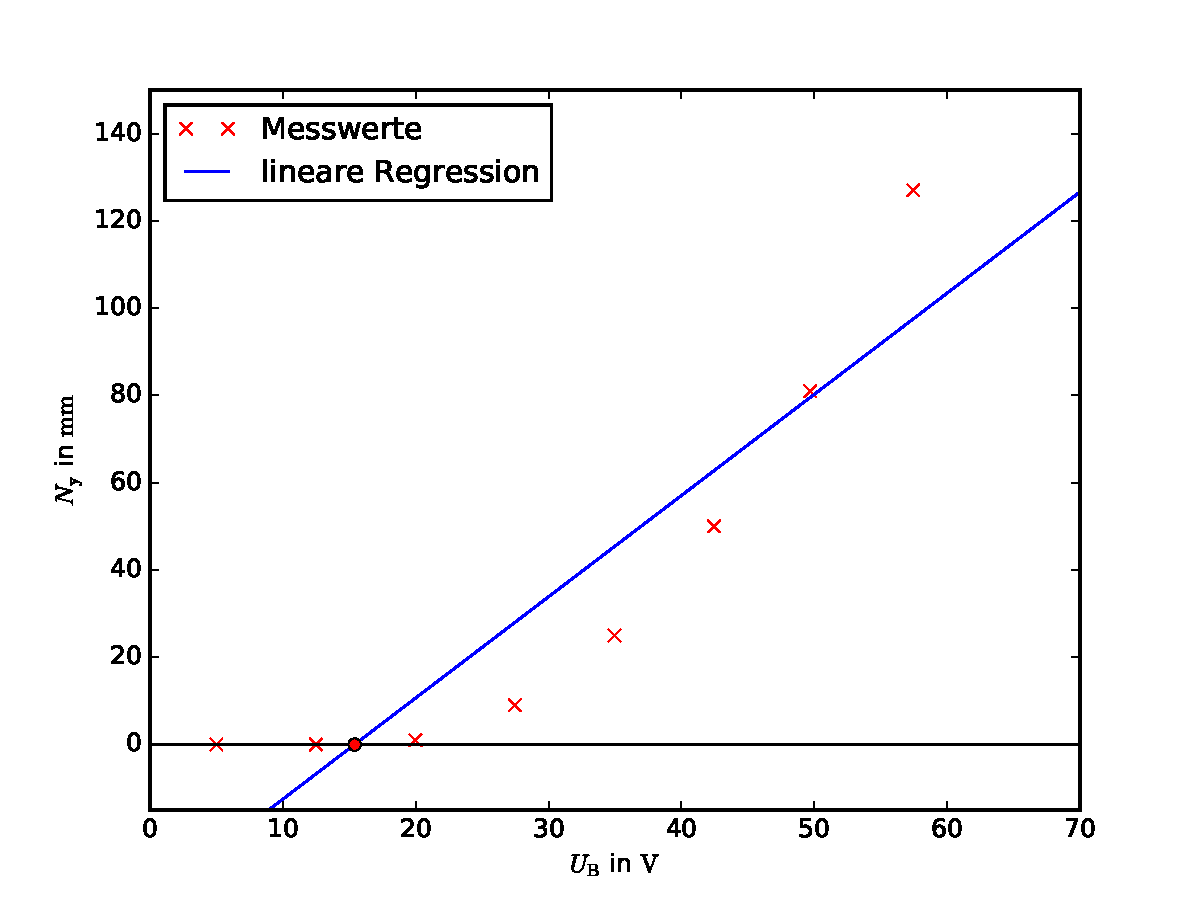
\includegraphics[width = \textwidth]{Pics/Ionisationsspannung.pdf}
  \caption{Lineare Regression durch die entnommen Messwerte.}
  \label{fig:MessungC}
\end{figure}

Mithilfe der linearen Regression ergibt sich die Nullstelle bei $U\ua{Null}$ =
15.4 $\si{V}$.
Mithilfe der Nullstelle kann nun die Ionisierungsspannung bestimmt werden, da
folgende Relation gilt:

\begin{equation}
  U\ua{ion} = U\ua{Null} - \su{K}.
\end{equation}

Verwendet man nun die beiden Kontaktpotentiale aus den Abschnitten 3.1 und 3.2,
ergeben sich für die Ionisierungsspannung folgende Werte:

\begin{align}
U\ua{ion,A} &= U\ua{Null} - \su{K}\ua{A} =  12.54 \si{V} \\
U\ua{ion,B} &= U\ua{Null} - \su{K}\ua{B} = (13.32 \pm 0.07) \si{V}.
\end{align}

\newpage

\section{Diskussion}

Ein Vergleich der beiden vom XY-Schreiber erstellten Graphen in Abschnitt 3.1
und der daraus resultierenden Energieverteilungen zeigt, dass bei der Messung
bei Raumtemperatur eine deutliche Abweichung von der Theoriekurve ersichtlich ist.
Theoretisch sollte eine Gauß-Kurve zu sehen sein. Jedoch ist die Steigung des
Graphen schon bei geringer Bremsspannung auffällig stark. Der Wendepunkt bei
$U\ua{B,eff}$ ist deshalb nicht deutlich ausgeprägt, jedoch schematisch erkennbar.

Bei der Messung 3.2 sind die Maxima der Franck-Hertz-Kurve deutlich ausgeprägt.
Die mit Hilfe der Abstände bestimmte Anregungsenergie von Quecksilber zeigt hierbei
eine Abweichung von lediglich 5 $\%$ im Vergleich zu dem Literaturwert\cite{Page02}:

\begin{align}
  E\ua{exp} &= \SI{5.160 \pm 0.035}{eV} \\
  E\ua{Lit} &= \SI{4.9}{eV} .
\end{align}

Auch hier wurde das Kontaktpotential erneut bestimmt, welches eine Abweichung von
ca. 27 $\%$ zu dem in Messung 3.1 bestimmten Kontaktpotential zeigt:

\begin{align}
  \su{K}\ua{A} &= \SI{2.853}{V} \\
  \su{K}\ua{B} &= \SI{2.08 \pm 0.07}{V} .
\end{align}

Die berechneten Kontaktpotentiale können jedoch nicht mit einem Literaturwert
verglichen werden.

Bei Messung 3.3 wurde zweimal die Ionisierungsspannung von Quecksilber bestimmt.
Im Vergleich mit dem Literaturwert $U\ua{ion,lit} = \SI{10.437}{V}$\cite{Page01}
ist unter Verwendung des Kontaktpotentials
aus Messung 3.1 eine kleinere Abweichung zu erkennen.

\begin{table}
  \centering
  \caption{Ergebnisse für die Ionisierungsspannung aus Messung 3.3 .}
  \label{tab:Ergebniss}
  \begin{tabular}{c c c}
    \toprule
    $\su{K}$ in $\si{V}$ & $U\ua{ion}$ in $\si{V}$ & (1 - $\sfrac{U\ua{ion,lit}}{U\ua{ion}}$) in $\%$ \\
    \midrule
    2.853 & 12.54 & 17 \\
    2.08  & 13.32 & 22 \\
    \bottomrule
  \end{tabular}
\end{table}

Unter Hinzuziehen des Kurvenverlaufs
des vom XY-Schreiber erstellten Graphen (siehe Anhang, Messung c) ) lässt sich sagen,
dass $\su{K}\ua{A}$ somit vermutlich näher am tatsächlichen Wert des Kontaktpotentials
liegt.

Für die auftretenden Abweichungen bei diesem Versuch gibt es mehrere Quellen.
Einerseits sollte bei dem Versuch bei jeder Messung der maximale Auffängerstrom
mit Hilfe des Speisestroms optimal eingestellt werden. Diese Variation war allerdings
nicht möglich, da der Speisestrom auf einen konstanten Kompromisswert eingestellt
war. Diese ermöglichte es, bei allen Messungen vernünftige Ergebnisse zu
erhalten, ohne Gefahr zu laufen, dass die Apparatur erheblich verstellt wird und
keine Messung mehr möglich ist. Jedoch wurde
die Qualität der Ergebnisse dadurch beeinflusst.

Eine weiter Fehlerquelle ist das Verbindungskabel zwischen der Franck-Hertz-Kammer
und dem Piccoamperemeter. Dieses sollte optimal isoliert sein, um
Störungen duch Induktionsströme zu vermeiden. Da das Kabel etwas älter war, kann
hier jedoch von einer auftretenden Störung ausgegangen werden.

Die nächste mögliche Störquelle ist die Regulierung des Temperatur. Aufgrund
äußerer Gegebenheiten kam es immer wieder zu Temperaturschwankungen, welche
zwar durch konstantes Regulieren der Temperatur gering gehalten werden sollten,
jedoch zusätzlich Auswirkungen auf die Qualität der Kurven hatten. Besonders bei
der Erstellung der Franck-Hertz-Kurve traten anfangs starke Temperaturschwankungen
auf, aufgrund derer mehrere Graphen angefertigt werden mussten. Bei allen Versuchen
wurde versucht, die Temperaturschwankungen im einem Fehlerintervall von ca. $\SI{1}{\su{K}}$
zu halten.

Zusammengefasst haben das Alter der Apparatur und die nicht variable Einstellung
des Speisestroms erhebliche Auswirkungen auf die Qualität des Experimentes
gehabt. Trotzdem ließen sich alle zu erwartenden Effekte in einem gewissen
Rahmen gut beobachten, was sich auch durch die nicht allzu hohen Abweichungen
der experimentell bestimmten Messwerte zu den Literaturwerten bestätigen lässt.
